\subsection{Gleichspannungswandler}
	Das Ziel von Gleichspannungswandlern ist es m�glichst verlustarm Gleichspannung entweder hoch- oder runterzuwandeln. Der Aufbau dieser Wandler ist wiefolgt:
	
	\subsubsection{Tiefsetzsteller(Buck-Converter)}
		Der Tiefsetzsteller arbeitet mithilfe von einem Schalttransistor, (meist ein MOSFET) welcher mit einem bestimmten Duty-Cycle(Tastgrad) ein- und ausgeschalten wird. Wenn der Schalter geschlossen ist, steigt der Strom durch die Induktivit�t langsam an und es flie�t kein Strom durch die Diode. Wenn der Schalter nun ge�ffnet wird, sinkt der Strom, der durch die Induktivit�t flie�t, linear ab und flie�t durch die Diode. Am Ausgang ist au�erdem ein Gl�ttungskondensator, um Spannungsspitzen auszugleichen. Wenn der Duty-Cycle des Schalttransistors ge�ndert wird, �ndert sich so die Ausgangsspannung.
	
	\begin{figure}[H]
		\centering
		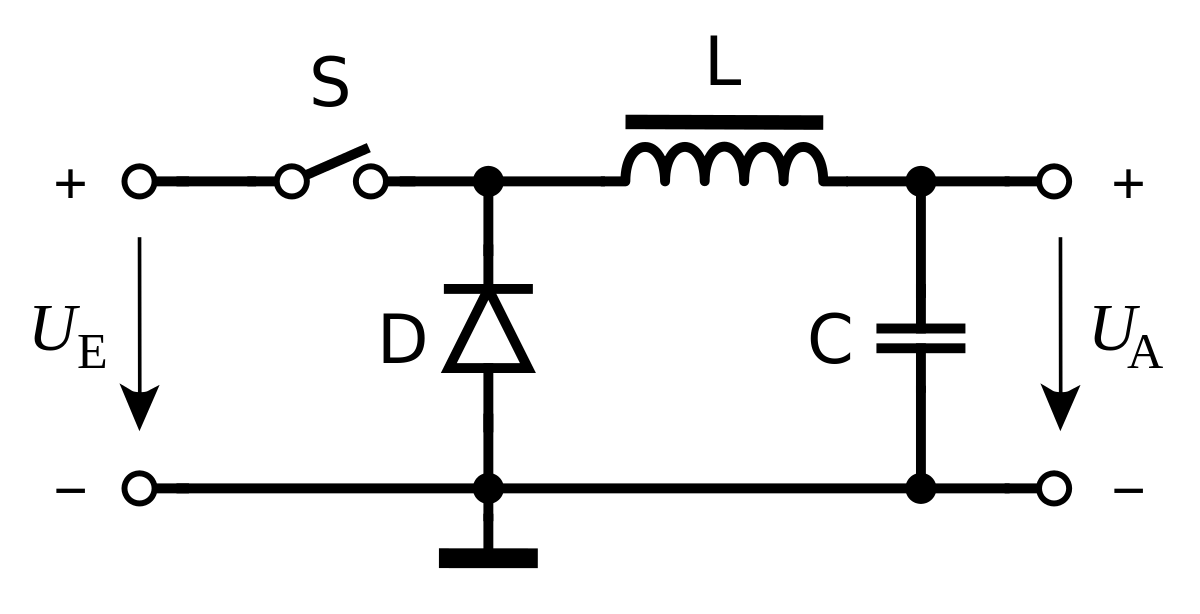
\includegraphics[scale=0.2]{./3_Stand_der_Technik/Abbildungen/Spannungswandler_1}
		\caption{Schaltbild eines Tiefsetzstellers\cite{wikipedia2024a}}
	\end{figure}
	
	\subsubsection{Hochsetzsteller(Boost-Converter)}
	Der Hochsetzsteller basiert auch auf einen Schalttransistor, der mit einem bestimmten Tastgrad ein- und ausgeschalten wird. Wenn der Schalttransistor geschlossen ist, f�llt die gesamte Eingangsspannung an der Diode ab, wird er nun ge�ffnet, sorgt die Induktivit�t daf�r, dass sich der Stromfluss nicht �ndert und die Spannung steigt an. Diese �berspannung l�dt nun den Kondensator am Ausgang h�her als die Eingangsspannung, danach widerholt sich der Vorgang.
	
	\begin{figure}[H]
		\centering
		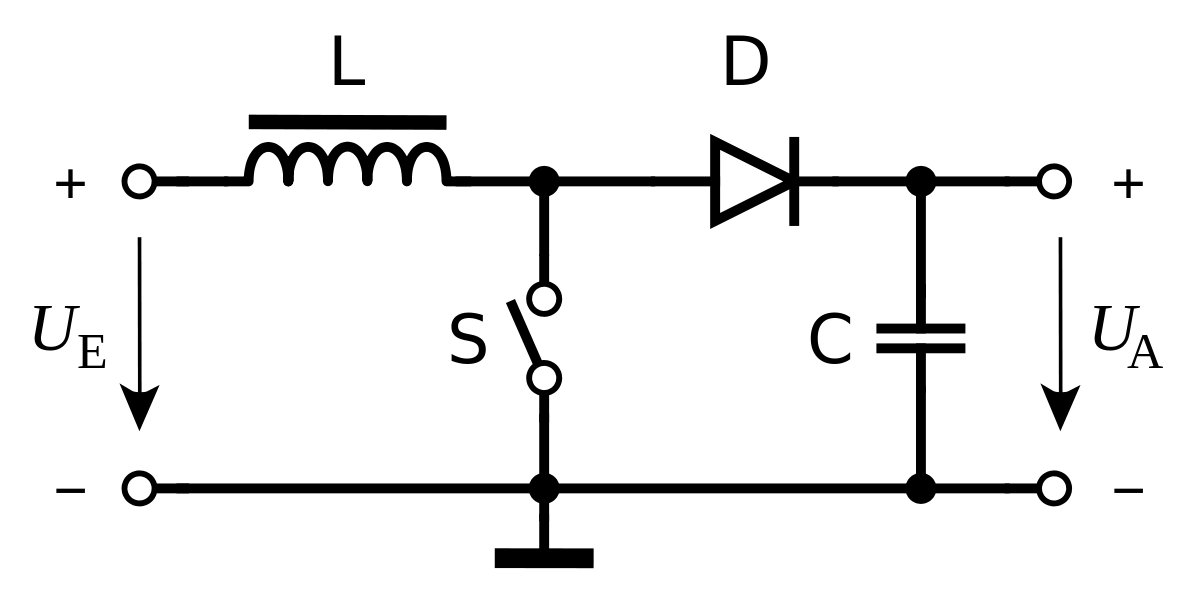
\includegraphics[scale=0.2]{./3_Stand_der_Technik/Abbildungen/Spannungswandler_2}
		\caption{Schaltbild eines Hochsetzstelers\cite{Wikipedia2024b}}
	\end{figure}
